\documentclass{beamer}
\title{Resumen T-$k^2$raster}
\subtitle{Vicente Lermanda Candia}

\usetheme{Simple}
\setbeamertemplate{frametitle}[default][center]
\begin{document}
	\frame {
		\titlepage
	}
	\frame {
		\centering
		{\Huge Related work}
	}
	\frame{
		\frametitle{\huge{Rank y select en bitmaps}}
		\centering
		\begin{itemize}
			\item {\huge Bitmap $B[0\ldots n]$ }
				\vspace*{1cm}
			\item {\huge $rank_a(B, i) $ }
				\vspace*{1cm}
			\item {\huge $select_a(B,i)$ }
		\end{itemize}
	}
	\frame{
		\frametitle{{\huge Quadtree}}
		\begin{figure}[h]
			\centering
			\hspace*{-0.5cm}
			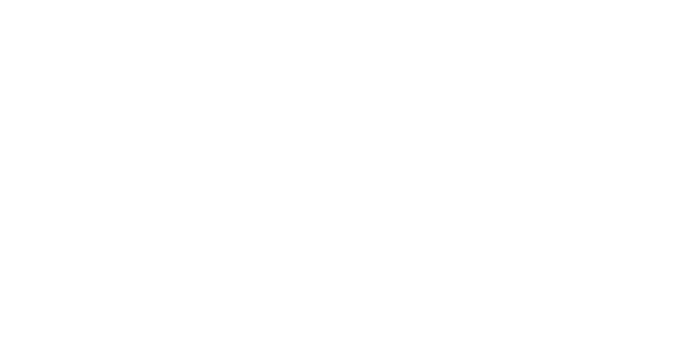
\includegraphics[width=1.1\textwidth]{images/quadp.png}
		\end{figure}
	}
	\frame{
		\frametitle{{\huge $k^2$tree}}
		\begin{itemize}
		\item {\LARGE Region quadtree. }
			\vspace*{1cm}
		\item {\LARGE Dos arreglos, $L$ y $T$. }
			\vspace*{1cm}
		\item {\LARGE $p_{hijos} = rank_1(T, p) \cdot k^2$ }
			\vspace*{1cm}
		\item {\LARGE Si $p_{hijos} > |T| \implies L[p_{hijos}-|T|]$}

		\end{itemize}

	}
	\frame{
		\frametitle{{\huge $k^3$tree}}
		\begin{figure}[h]
			\centering
			\hspace*{-0.5cm}
			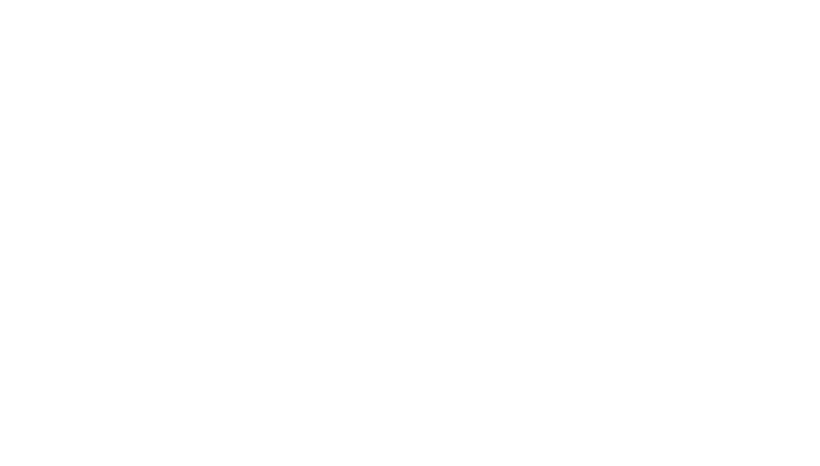
\includegraphics[width=1.1\textwidth]{images/k3treep.png}
		\end{figure}
	}
	\frame{
		\centering
		{\Huge Representación compacta de rasters}
	}
	\frame{
		\frametitle{{\huge $k^2$raster}}
	\begin{itemize}
		\item {\Large Matrices de enteros.}
			\vspace*{0.5cm}
		\item {\Large Nodos almacenan máximos y mínimos. }
			\vspace*{0.5cm}
		\item {\Large Subdivisión hasta que max y min sean iguales, o hasta llegar a
			una celda.}
			\vspace*{0.5cm}
		\item {\Large Arreglo de bits $T$.}
			\vspace*{0.5cm}
		\item {\Large Codificación diferencial.}
			\vspace*{0.5cm}
		\item {\Large $Lmax$ y $Lmin$.}

	\end{itemize}
	}
	\frame{
		\begin{figure}[h]
			\centering
			\vspace*{-0.3cm}
			\hspace*{-0.6cm}
			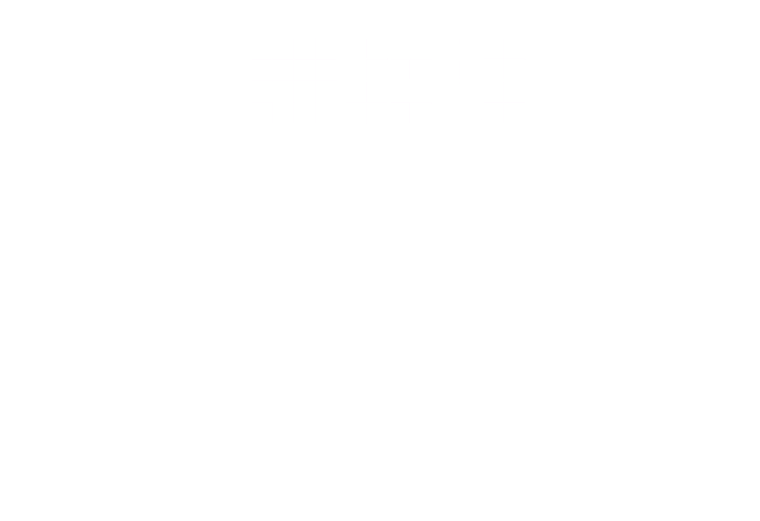
\includegraphics[width=1.1\textwidth]{images/k2rasterp.png}
		\end{figure}
	}
	\frame{
		\frametitle{{\huge 3D2D-mapping}}
		\begin{itemize}
			\item {\large Matriz raster $\to$ matriz binaria.}
		\end{itemize}
		\vspace*{0.4cm}
		\hspace*{1.5cm}
		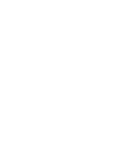
\includegraphics[width=0.13\textwidth]{images/z.png}
		\begin{figure}[h]
			\centering
			\vspace*{-1.1cm}
			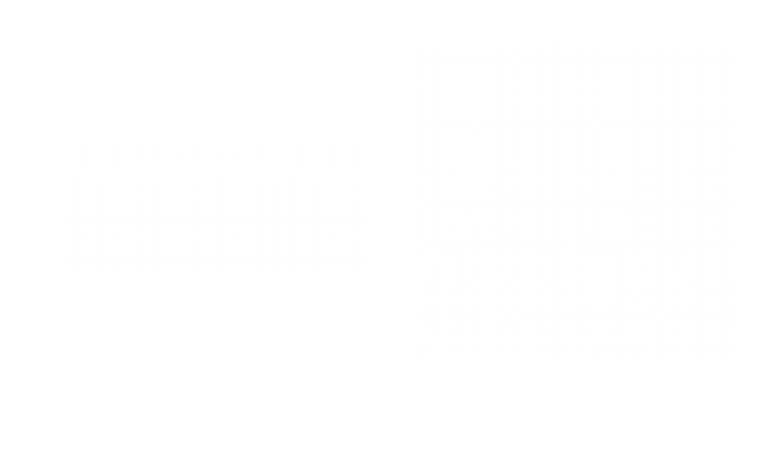
\includegraphics[width=0.8\textwidth]{images/3d2dp.png}
		\end{figure}
	}
	\frame{
		\centering
		{\Huge Representación compacta de rasters time series}
	}
	\frame{
		\frametitle{{\huge 4D3D-mapping}}
		\begin{figure}[h]
			\centering
			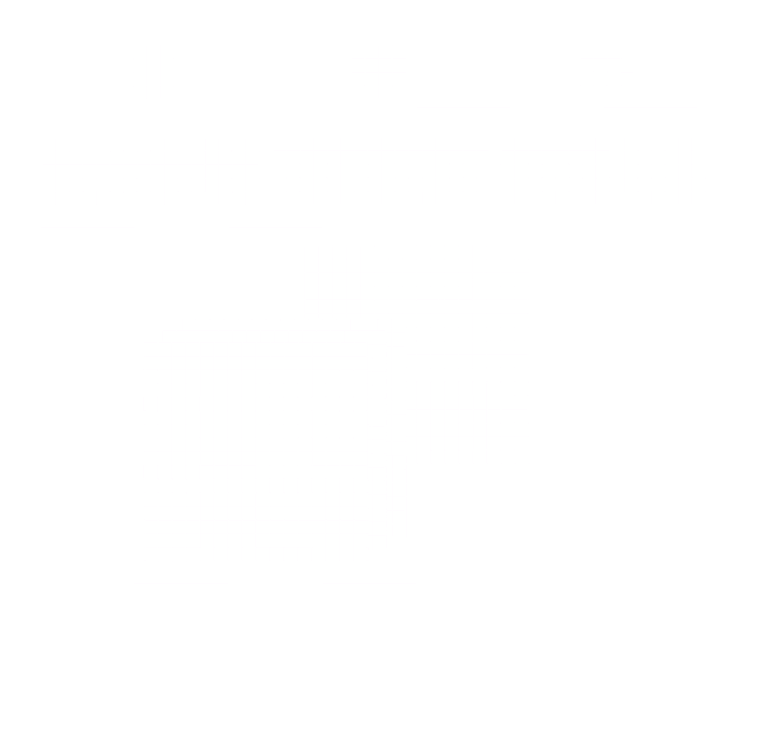
\includegraphics[width=1.0\textwidth,height=8.3cm]{images/4d3dp.png}
		\end{figure}
	}
	\frame{
		\vspace*{-0.5cm}
		\centering
		{\Huge Problem definition}
		\vspace*{1.7cm}
\begin{itemize}
  \item {\large Tenemos una secuencia de matrices raster para distintos
			instantes de tiempo $\tau$. Asumimos que cada celda de los raster
		almacena un entero.}
\end{itemize}
	}
	\frame{
		\frametitle{{\huge Querys}}
		\begin{itemize}
		\item {\Large $access(r,c,t)$}
			\vspace*{1.1cm}
		\item {\Large $windowQuery(r_1, r_2, c_1, c_2, t_1, t_2)$}
			\vspace*{1.1cm}
		\item {\Large $rangeQuery(r_1, r_2, c_1, c_2, t_1, t_2, rMin, rMax)$}
		\end{itemize}
	}

	\frame{
		\frametitle{{\huge q-cols \& q-rows}}
		\vspace*{-0.3cm}
		\begin{figure}[h]
			\centering
			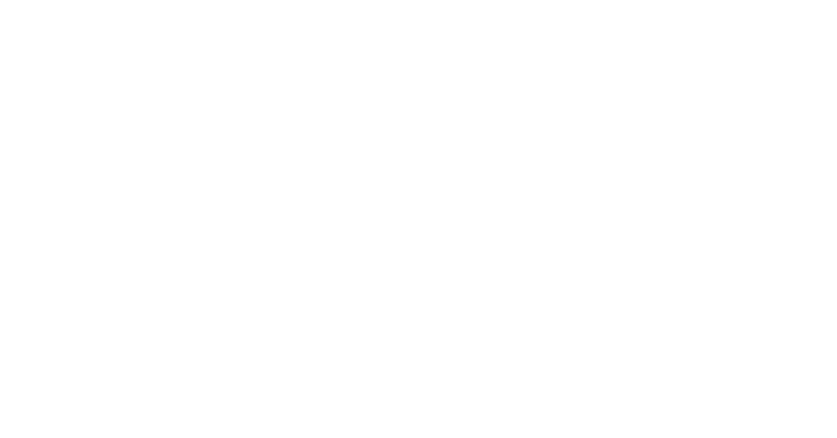
\includegraphics[width=0.7\textwidth]{images/qrowp.png}
		\end{figure}
		\vspace*{-0.3cm}
		\begin{itemize}
		 \item {\small Dada una q-row, q-row$_i$ y la fila original $r  |
				 r \in \{0,\ldots,n-1\}$, definimos $relative\_row(\text{q-row}_i,r)$
				 de la siguiente forma:}
				\begin{itemize}
					\item {\small Si $r \in q-row_i$, retorna la posición relativa de $r$
							dentro de q-row$_i$.}
					\item{\small Si $r$ está en una q-row anterior a q-row$_i$, retorna 0.
					\item Si $r$ está en una q-row posterior a q-row$_i$, retorna
					$\frac{n}{k}-1$.}
				\end{itemize}
			\item {\small La función $relative\_col(q-col_i, r)$ funciona de manera análoga.}
		\end{itemize}
	}
	\frame{
		\frametitle{{\huge T-$k^ 2$raster}}
		\begin{itemize}
			\item {\Large Snapshots y logs.}
				\vspace*{0.6cm}
			\item {\Large Matrices $M_t$ y $M_s$.}
				\vspace*{0.6cm}
			\item	{\Large $s = i + 1\cdot t_\delta, i \in [0,(\tau - 1) / t_\delta] $.}
				\vspace*{0.6cm}
			\item {\Large $t \in [s+1, s+t_\delta -1]$.}
				\vspace*{0.6cm}
			\item {\Large Para representar $M_t$ se usa $k^2$raster'.}
		\end{itemize}
	}

	\frame{
		\frametitle{{\huge $k^ 2$raster'}}
		\begin{itemize}
			\item {\large Codificado en base a las diferencias con $M_s$.}
				\vspace*{0.5cm}
			\item {\large Bitmap $eqB$.}
				\vspace*{0.5cm}
			\item {\large Sea $\alpha \gets maxval_t - maxval_s$.}
				\vspace*{0.5cm}
			\item {\large Si llegamos a las celdas, $Lmax[z_t_j] \gets \alpha$.}
				\vspace*{0.5cm}
			\item {\large Si $maxval_t == minval_t$, $T_t[z_t_j] \gets 0$,
				$eqB[rank_0(T_t,z_t_j)] \gets 0$ y $Lmax[z_t_j] \gets \alpha$.}
				\vspace*{0.5cm}
			\item {\large Si $q_t_j$ y $q_t_s$ difieren por completo en $\alpha$,
				$T_t[z_t_j] \gets 0$, $eqB[rank_0(T_t,z_t_j)] \gets 1$ y
			$Lmax[z_t_j] \gets \alpha$.}
		\end{itemize}
	}
	\frame{
		\begin{figure}[h]
			\centering
			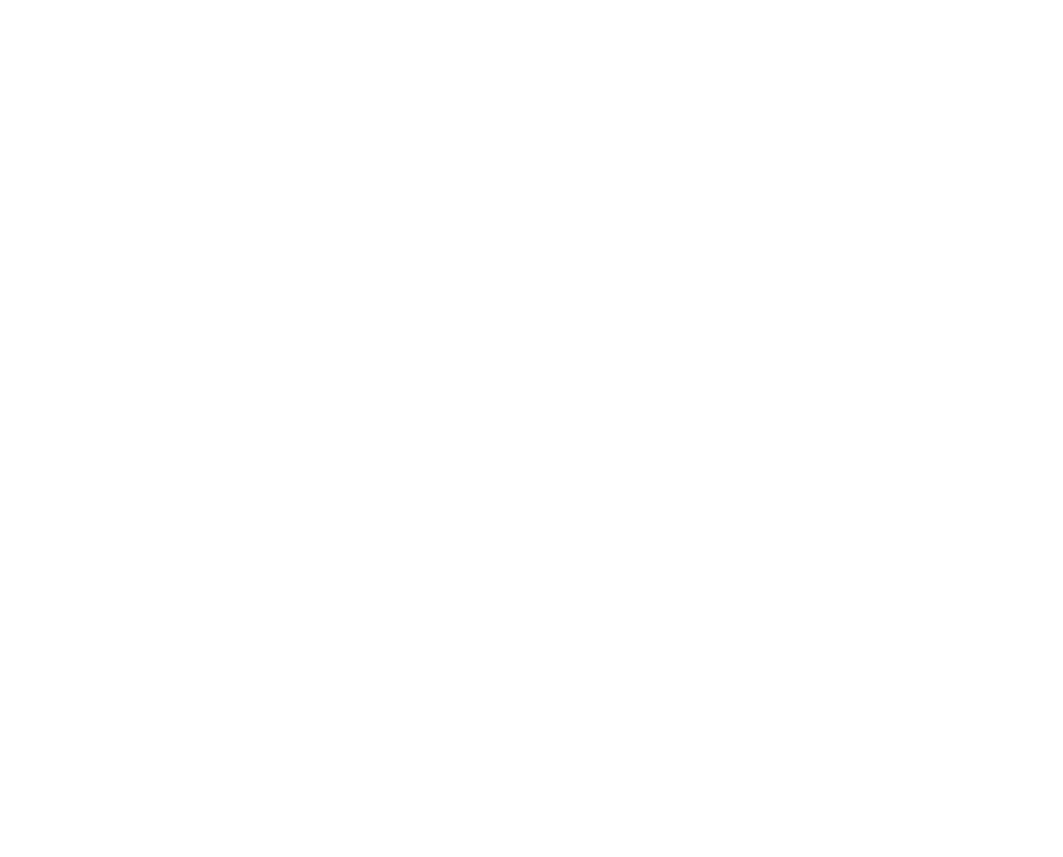
\includegraphics[width=1.0\textwidth]{images/tk2.png}
		\end{figure}
		\clearpage
	}
	\frames{
		\frametitle{\huge{Querying}}

	}

\end{document}
